\documentclass[times, utf8, seminar]{fer}
\usepackage{algorithmic}
\usepackage{algorithm}
\usepackage{booktabs}
\usepackage{listings}
\usepackage{xcolor}
\newcommand\myworries[1]{\textcolor{red}{#1}}
\usepackage{hyperref} 
\usepackage{natbib}
\usepackage{subfig}
\usepackage{color}
\usepackage{placeins}
\usepackage{multirow}

\definecolor{mygreen}{rgb}{0,0.6,0}
\definecolor{mygray}{rgb}{0.5,0.5,0.5}
\definecolor{mymauve}{rgb}{0.58,0,0.82}
\renewcommand\labelitemi{•}

\lstset{ %
  backgroundcolor=\color{white},   % choose the background color
  basicstyle=\footnotesize,        % size of fonts used for the code
  breaklines=true,                 % automatic line breaking only at whitespace
  captionpos=b,                    % sets the caption-position to bottom
  commentstyle=\color{mygreen},    % comment style
  escapeinside={\%*}{*)},          % if you want to add LaTeX within your code
  keywordstyle=\color{blue},       % keyword style
  stringstyle=\color{mymauve},     % string literal style
}
\begin{document}


\title{Međujezično prepoznavanje imenovanih entiteta pomoću wikifikacije}

% TODO: Navedite vaše ime i prezime.
\author{Stipan Mikulić}
\voditelj{dr. sc. Jan Šnajder}

\maketitle

\tableofcontents

\chapter{Uvod}
U današnje vrijeme svjedočimo stalni eksponencijali porast svih vrsta podataka, naročito teksta. Zbog tog naglog porasta podataka ljudi više nisu u mogućnosti obraditi te podatke da bi prepoznali bitne i korisne informacije. Riješenje problema krije se u računalnoj obradi podataka. 
Ovim problemom se bavi područje računarske znanosti (engl. computer science), umjetne inteligencije (engl. artificial intelligence) i strojnog učenja (engl. machine learning) koje se naziva obrada prirodnog jezika (engl. natural language processing, NLP). \\
\indent U ovom radu razvit će se model za međujezično prepoznavanje imenovanih entiteta. Za razvoj dobrog modela za klasifikaciju potrebno nam je puno podataka. Prema zadnjim procjenama više od $ 50\% $ sadžaja na internetu je pisano na engleskom jeziku.\footnote{\url{https://en.wikipedia.org/wiki/Languages_used_on_the_Internet}}U potpunoj dominaciji engleskog jezika u svim vrstama podataka i NLP alata i leži motivacija za razvoj međujezičnog modela. \\
\indent Rad je strukturiran tako da u drugom poglavlju opisuje problem, u trećem analizira podatke nad kojima treniramo, validiramo i testiramo model. Četvrto poglavlje opisat će sam model za prepoznavanje imenovanih entiteta, a peto implementciju tog modela. Rezultati i evaluacija će biti opisani u šestom poglavlju. Zadnjem poglavlje će dati kratki zaključak rada.
\chapter{Opis problema}

Prepoznavanje imenovanih entiteta je zadatak ekstrakcije informacija kojem je cilj klasificirati i locirati elemente u predefinirane kategorije kao što su:

\begin{itemize}
	\item Imena -- Osobe, Organizacije, Lokacije
	\item Vremena -- Vrijeme, Datum
	\item Brojevi -- Novac, Postotci
\end{itemize}

Iako su kategorije unaprijed definirane i dalje se postavlja pitanje koliko općenite i obuhvatne trebaju biti. Ovisno o domeni za koju se koriste imenovani entiteti, moguće ih je prizvoljno definirati. Pogledajmo pobliže ovaj problem kroz primjer. Ako sustavu za prepoznavanje imenovanih entiteta damo sljedeći tekst kao ulaz: \\\\
\centerline{Jim  bought 300 shares of Acme Corp. in 2006.}\\\\
na izlazu statava ćemo dobiti:\\\\
\centerline{[Jim]\textsubscript{OSOBA} bought [300]\textsubscript{BROJ} shares of [Acme Corp.]\textsubscript{ORGANIZACIJA} in [2006]\textsubscript{VRIJEME}.}\\\\
U ovom primjeru entitet OSOBA sadrži jedan token dok entitet ORGANIZACIJA sadrži dva tokena.\footnote{\url{https://en.wikipedia.org/wiki/Named-entity_recognition}} U ovom radu želimo prepoznati sljedeće entitete u tekstu:

\begin{itemize}
	\item PER -- Osobe
	\item ORG -- Organizacije
	\item LOC -- Lokacije
	\item MISC -- Razno
\end{itemize}

\newpage 

Najčešći pristup ovom problemu je uz pomoć metoda nadziranog strojnog učenja. Ovaj problem spada u kategoriju označavanja slijedova (engl. sequence labeling) gdje se svakom članu slijeda pridružuje neka oznaka tj. predefinirana kategorija. Oznake su ovisne o svim članovima oko njih u slijedu. Zbog toga se ovisnost izražava s lijeva na desno, s desna na lijevo ili zajednički. Radi boljeg razumjevanja problema u idućem poglavlju će se pisati o analizi podataka.

\chapter{Analiza podataka}
Model za međujezično prepoznavanje imenovanih entiteta razvijen je nad skupovima podataka iz CoNLL02 i CoNLL03 dijeljenog zadatka. Skup podataka uključuje podatke na engleskom, španjolskom i nizozemskom jeziku. CoNLL skup podataka je podskup novinskih članaka Reutersa iz 1996. Entiteti su označeni u 4 razreda: PER, ORG, LOC i MISC. Skup za treniranje su članci iz kolovoza 1996, dok je testni skup iz prosinca 1996. Imenovani entiteti u testnom skupu su znatno različiti od skupa za treniranje što ih čini značajno težim.\citep{Ratinov:2009:DCM:1596374.1596399} \\
\indent Španjolski i nizozemski skup podataka označen je BIO\footnote{Format u kojem se s B (\textbf{B}egining) označavaju riječi na početku entiteta, I (\textbf{I}nside) označavaju riječi unutar entiteta i O (\textbf{O}utside) označavaju riječi koje ne pripadaju ni jednom entitetu.} formatom dok je engleski skup podataka označen IO formatom\footnote{Format u kojem se s I (\textbf{I}nside) označavaju riječi koje pripadaju nekom entitetu i O (\textbf{O}utside) označavaju riječi koje ne pripadaju ni jednom entitetu.} koji je naknadno pretvoren u BIO.
\begin{center}
\captionof{table}{Broj entiteta u skupovima}
\begin{tabular}{ clcccc }
\hline
\textbf{language} & \textbf{set} & \textbf{PER} & \textbf{ORG} & \textbf{LOC} & \textbf{MISC} \\ \hline
\multirow{3}{*}{eng} & train & 6600 & 6321 & 7140 & 3438 \\
 & validation & 1842 & 1341 & 1837 & 922 \\
 & test & 1617 & 1661 & 1668 & 702 \\ \hline
\multirow{3}{*}{esp} & train & 4321 & 7390 & 4913 & 2173 \\
 & validation & 1222 & 1700 & 984 & 445\\
 & test & 735 & 1400 & 1084  & 339 \\ \hline
\multirow{3}{*}{ned} & train & 4716 & 2082 & 3208 & 3338 \\
 & validation & 703 & 686 & 479 & 748 \\
 & test & 1098 & 882 & 774 & 1187 \\ \hline
\end{tabular}
\end{center}
\newpage

\begin{center}
  \makebox[\textwidth]{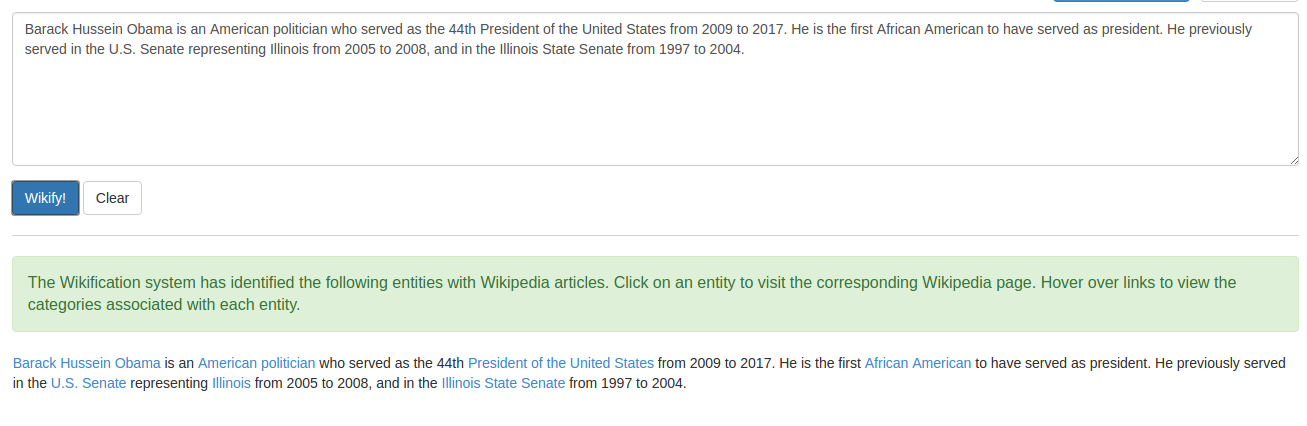
\includegraphics[scale=0.4]{images/eng.png}}
\captionof{figure}{Veličina entiteta skupa podataka na engleskom jeziku}

\end{center}

\begin{center}
  \makebox[\textwidth]{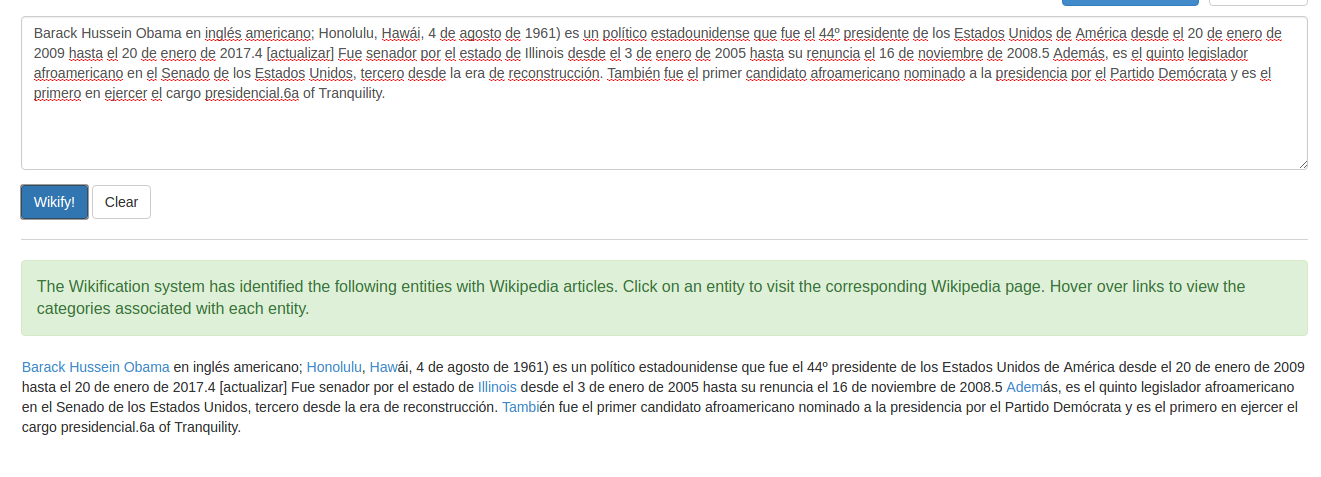
\includegraphics[scale=0.4]{images/esp.png}}
\captionof{figure}{Veličina entiteta skupa podataka na španjolskom jeziku}
\end{center}

\begin{center}
  \makebox[\textwidth]{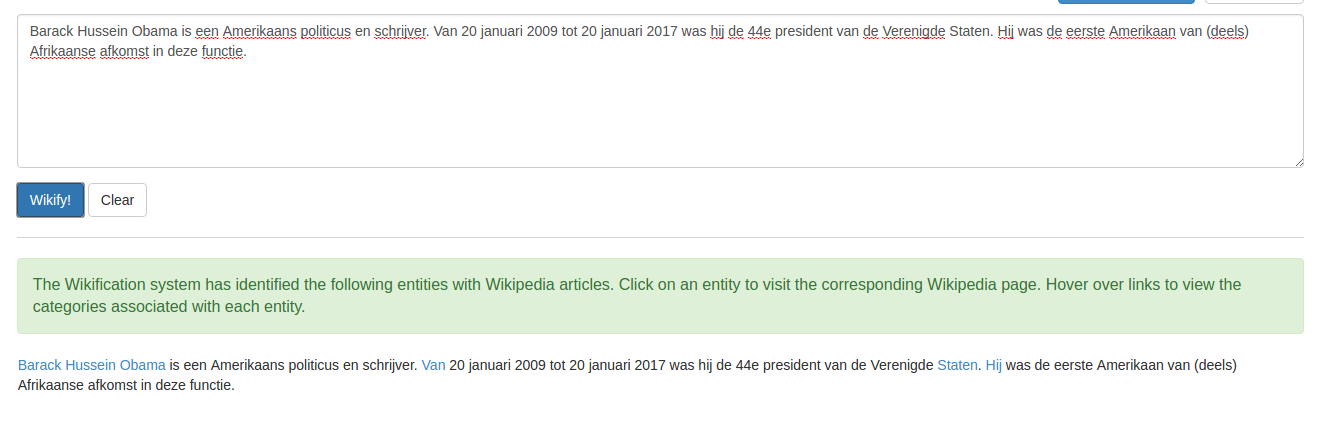
\includegraphics[scale=0.4]{images/ned.png}}
\captionof{figure}{Veličina entiteta skupa podataka na nizozemskom jeziku}
\end{center}
\chapter{Model}
\section{Perceptron}
U svrhu prepoznavanja imenovanih entiteta u tekstu najčešće se koriste sljedeći modeli: 
\begin{itemize}
\item HMM (Hidden Markov Model)
\item CRF (Conditional random field)
\item MaxEnt
\item Perceptron
\end{itemize}

U ovom radu korišten je Perceptron. Iako prva dva navedena modela daju mogućnost zajedničkog učenja oznaka u slijedu, ipak je korišten Perceptron koji nam omogućuje korištenje raznih značajki.

\indent Perceptron je matematički model neurona. U stvarnom neuronu dendriti dobivaju signale od aksona drugih neurona dok su u matematičkom modelu dendriti predstavljeni s brojčanim vrijednostima. Izlaz neurona, akson, predstavljen je aktivacijskom funkcijom koja kao argument prima težinsku sumu ulaza neurona zbrojenom s pomakom.\footnote{\url{https://cs.stanford.edu/people/eroberts/courses/soco/projects/neural-networks/Neuron/index.html}}. Najčešće korištena aktivacijska funkcija je $ sigmoid $\footnote{\url{https://en.wikipedia.org/wiki/Sigmoid_function}}.
\[ suma = \sum_{i=1}^{n} w_ix_i + b\]
\[ izlaz = sigmoid(suma) \]
Perceptron pokušava naučiti težine na način da ih ne ažurira nakon prolaska kroz cijeli skup podataka već nakon svakog primjera. Ovakav način učenja se zove online učenje.  
\newpage
\begin{center}
  \makebox[\textwidth]{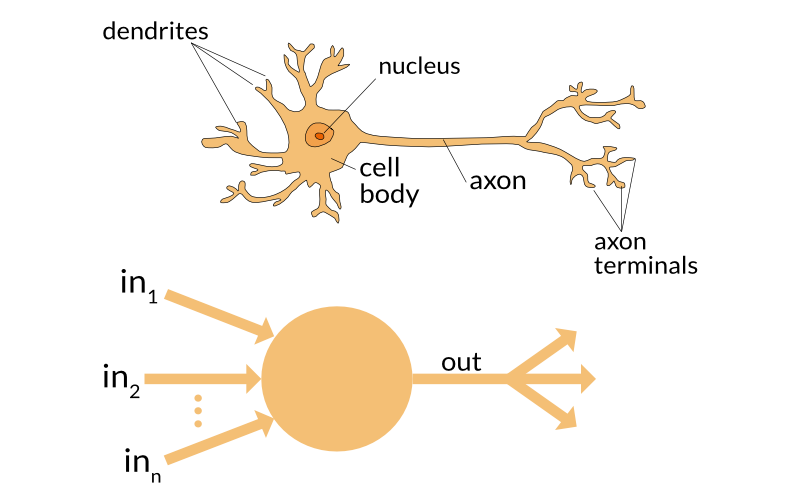
\includegraphics[scale=0.4]{images/neuron.png}}
\captionof{figure}{Matematički model biološkog neurona}\footnote{\url{https://appliedgo.net/perceptron/}}
\end{center}
\section{Logistička regresija}


\chapter{Implementacija modela}
\myworries{cross validacija, baseline, obicne znacajke, gazetteri-grupe, wikifikacija, 9-class clasification, klase}
Sustav za prepoznavanje imenovanih entiteta je razvijen u programskom jeziku Python3. Korištena je implementacija Perceptrona iz scikit-learn\footnote{\url{http://scikit-learn.org/stable/modules/generated/sklearn.linear_model.Perceptron.html}} knjižnice. 
Glavni program runner.py pokreće cijeli cjevovod sustava. Moguće je specificirati jezike skupa za treniranje, validaciju i testiranje preko argumenata komandne linije. Naredba za pokretanje programa koji trenira i validira sustav engleskim i nizozemskim jezikom a testira nad španjolskim jezikom.
\begin{center}
python3 runner.py -train eng,ned -validation eng,ned -test esp
\end{center}

Nakon parsiranja argumenata dohvaćaju se navedeni skupovi za treniranje, validiranje i testiranje. Nakon toga se izvlače značajke iz podataka te se pretprocesiraju u brojčani oblik pogodan za algoritam. Prilikom odabira najboljeg modela radi se unakrsna validacija nad skupovima za treniranje i validiranje. 

Razvijena su tri modela koji se razlikuju u značajkama:
\begin{enumerate}
\item Osnovni model (engl. baseline) 
\item Osnovni model + Gazeteri
\item Osnovni model + Gazeteri + Wikifikacija
\end{enumerate}
\textbf{Gazeteri} su unaprijed prikupljeni skupovi entiteta. Za potrebe ovog modela prikupljeni gazeteri su podijeljeni u teme čiji su naslovi korišteni kao značajke modela. Neke od tema su: ArtWork, Building, Clothes, Films, Parks, Vehicles itd. Dodatno su prikupljeni skupovi za entitete Osoba, Organizacija i Lokacija te su za značajke korišteni kao broj pojavljivanja riječi u pojedinom skupu. Za dohvaćanja teme za neku riječ korišten je pomični prozor veličine $ 4 $. Ovisno o poziciji na kojoj se nalazi riječ u prozoru dodaje se prefiks B- ili I- temi kojoj pripada. Ako neka riječ ima više tema kojima pripada biramo prvu nađenu.\citep{DBLP:conf/conll/TsaiMR16}
\newpage
\myworries{opisati wikifikaciju}

\begin{center}
\captionof{table}{Statistika gazetera i wiki-a}
\begin{tabular}{ lcccc }
\hline
 & PER & LOC & ORG & MISC\\ 
\hline
Gazeteri & 2 972 k & 3 106 k & 977 k & 2 991 k \\
Wiki & -- & -- & -- & -- \\
\hline
\end{tabular}
\end{center}



\section{Značajke}
U tablici je naveden popis značajki podjeljen prema modelima u kojima su korištene.

\begin{center}
\captionof{table}{Značajke sustava}
\begin{tabular}{llr}
\hline
\textbf{Osnovne značajke} & \\
prethodni tag entiteta & $ (t_{i-1},t_{i-2}) $\\ 
sadrži samo brojke i slova & $ alphanumeric(w_i) $\\ 
sadrži samo brojke  & $ alldigits(w_i) $\\ 
sadrži samo veika slova & $ allcaps(w_i) $\\ 
sadrži samo brojke & $ iscapitalized(w_{i-2}, w_{i-1}, w_{i}, w_{i+1}, w_{i+2}) $\\
3-gram & suma pojavljivanja 3-grama za svaku klasu \\
\textbf{Gazeteri} & \\
naziv kategorije gazetera  & $ topic(w_{i}, w_{i+1}, w_{i+2}, w_{i+3}) $\\
\textbf{Međujezične značajke} & \\
\hline
\end{tabular}
\end{center}


\myworries{detaljnije opisati znacajke, dodati trigram znacajke}
\section{Pretprocesiranje značajki}
Većina korištenih značajki su kategoričke stoga su kodirane Onehot \footnote{Svaka kategorija neke značajke se kodira u vektor duljine $ broj\_kategorija $ tako da je jedan element vektora $ 1 $ a ostali $ 0 $. \url{http://scikit-learn.org/stable/modules/generated/sklearn.preprocessing.OneHotEncoder.html}} metodom. Brojčane značajke kojima je definiran poredak skalirane su na interval $ [0,1] $. Za skaliranje je korišten MinMaxScaler\footnote{\url{http://scikit-learn.org/stable/modules/generated/sklearn.preprocessing.MinMaxScaler.html\#sklearn.preprocessing.MinMaxScaler}}.
\section{Unakrsna validacija}
Unaksrsna 5-struka validacija je korištena radi dobivanja najboljeg mogućeg modela za dane podatke. Parametri perceptrona koji su optimizirani unakrsnom validacijom: 

\[ alpha = (10^{-10}, 10^{-9}, ..., 10^{-2}) \]
\[ penalty = (l2, l1) \]

oba parametra se koriste u svrhu regularizacije,  alpha je konstanta koja množi regularizacijski faktor a penalty je regularizacijska funkcija.
\chapter{Evaluacija}
\myworries{evaluacijske mjere, tablice s rezultatima, exact evaluacija, corelation matrix za evaluaciju}

Evaluacija sustava rađena je nad testnim skupom podataka. Model koji evaluiramo je najbolji model dobiven unakrsnom validacijom. Mjere koje su korištene za evaluaciju su f1-score, precision, recall, micro and macro accuracy.

\begin{center}
\captionof{table}{Evaluacijske mjere}
\begin{tabular}{ lcccccccc }
\hline
& \multicolumn{4}{c}{Perceptron} & \multicolumn{4}{c}{Log. regresija} \\ 
\cline{2-5}\cline{6-9}
 & ENG & ESP & NED & AVG & ENG & ESP & NED & AVG\\ 
\hline
Entiteti (treniranje) & -- & -- & -- & -- & -- & -- & -- & -- \\
Entiteti (testiranje) & -- & -- & -- & -- & -- & -- & -- & -- \\
\hline
\multicolumn{19}{c}{Jednojezični eksperimenti } \\
\hline
Osnovne značajke & -- & -- & -- & -- & -- & -- & -- & -- \\
+Gazeteri & -- & -- & -- & -- & -- & -- & -- & -- \\
+Wikifikacija & -- & -- & -- & -- & -- & -- & -- & -- \\
\hline
\multicolumn{9}{c}{Međujezični eksperimenti } \\
\hline
Osnovne značajke & -- & -- & -- & -- & -- & -- & -- & -- \\
+Gazeteri & -- & -- & -- & -- & -- & -- & -- & -- \\
+Wikifikacija & -- & -- & -- & -- & -- & -- & -- & -- \\
\hline
\end{tabular}
\end{center}
\section{Poboljšanja}
	presjek tema za gazettere
\chapter{Zaključak}
\myworries{zakljuciti}
\bibliographystyle{fer}
\bibliography{literatura}
\nocite{*}

\begin{sazetak}

Zbog stalnog rasta svih vrsta podataka, naročito teksta ljudi više nisu u mogućnosti obraditi te podatke da bi prepoznali bitne i korisne informacije. Zbog toga posežemo za računalnom obradom podataka. U ovom radu razvijen je model za međujezično prepoznavanje imenovanih entiteta. Za razvoj dobrog modela za klasifikaciju potrebno nam je puno podataka. Prema zadnjim procjenama više od $ 50\% $ sadžaja na internetu je pisano na engleskom jeziku. Motivacija za razvoj međujezičnog modela leži u potpunoj dominaciji engleskog jezika u svim vrstama podataka i NLP alata. Razvojem takvog modela jezici sa skromnim izvorima podataka bi napredovali ne samo u prepoznavanju imenovanih entiteta već u analizi teksta općenito.

\kljucnerijeci{Strojno učenje, Procesiranje prirodnog jezika, Prepoznavanje imenovanih entiteta, Perceptron}
\end{sazetak}
% TODO: Navedite naslov na engleskom jeziku.
\engtitle{Cross-Lingual Named Entity Recognition via Wikification}
\begin{abstract}
Because of the steady growth of all kinds of data, especially text, people are no longer able to process this data to recognize essential and useful information. That's why we reach for computer data processing. In this paper, a model for cross-lingual named entity recognition was developed. To develop a good model for classification we need a lot of data. According to the latest estimates, more than $ 50 \% $ of web content is written in English. Motivation for the development of an cross-lingual model lies in the overall dominance of English in all types of data and NLP tools. By developing such a model, languages with modest data sources would advance not only in the recognition of named entities, but in text analysis in general.


\keywords{Machine learning, Natural language processing, Named entity recognition, Perceptron}
\end{abstract}

\end{document}
